\documentclass[a4paper,11pt]{article}
\usepackage[utf8]{inputenc}
\usepackage{fullpage}
\usepackage{color}
\usepackage{authblk}
\usepackage{listings}
\usepackage{graphicx}
\usepackage{subfigure}

\definecolor{codegreen}{rgb}{0,0.6,0}
\definecolor{codegray}{rgb}{0.5,0.5,0.5}
\definecolor{codepurple}{rgb}{0.58,0,0.82}
\definecolor{backcolour}{rgb}{0.95,0.95,0.92}
 
%opening
% \address{$^{\text{\sf 1}}$Synthetic Biology Research Centre, University of Nottingham, Nottingham, NG7 2RD, United Kingdom and \\
% $^{\text{\sf 2}}$Intelligent Modelling and Analysis group, School of Computer Science, University of Nottingham, Nottingham, NG7 2RD, United Kingdom}



\title{Gsmodutils: A python based framework for test driven genome scale metabolic model development}
\author[1]{James Gilbert}
\author[1]{Nicole Pearcy}
\author[2]{Jamie Twycross}
\affil[1]{Synthetic Biology Research Centre, University of Nottingham, Nottingham, NG7 2RD, United Kingdom}
\affil[2]{Intelligent Modelling and Analysis group, School of Computer Science, University of Nottingham, Nottingham, NG7 2RD, United Kingdom}

\begin{document}

\maketitle

\begin{abstract}
\textbf{Motivation:} Genome scale metabolic models are increasingly important for systems biology and metabolic engineering research, capable of simulating complex steady state phenotypic behaviour.
Models of this scale can include thousands of reactions and metabolites, with many crucial pathways that only become activated in specific simulation settings.
However, despite their widespread use, power and the availability of tools to aid with the construction and analysis of large scale models, little methodology is suggested for the management of continually curated large scale models.\\
\textbf{Results:} Taking advantage of python and cobrapy integration, we have developed the \textit{gsmodutils} modelling framework.
As a fully documented python API and series of command line utilities, gsmodutils places an emphasis on test driven design of models through easy to write test cases in json or python.
Crucially, different substrate conditions are configurable allowing users to examine how different designs or curation impact a wide range of system behaviours, hopefully, minimising error between model versions. \\
Furthermore, a core feature of the software is to allow users to easily create shareable, self contained, docker images that can be run in cross platform environments.\\
\textbf{Availability:} The software framework described within this paper is open source and freely available from http://github.com/gsmodutils \\
\textbf{Contact:}{jamie.twycross@nottingham.ac.uk}
\end{abstract}


\section{Introduction}
Constraints based modelling for biological systems has become a mainstay of systems biology for several decades.
More recently, the structural approach has become a popular method for modelling steady state behaviour of large, metabolic networks.
Such large scale reconstructions are often refereed to as genome scale models (GSMs), as the processes is significantly aided throught the advent of genome sequencing.

The reconstruction of GSMs is an arduous process that follows a complex protocol to ensure model validity \cite{thiele2010protocol}.
Whilst many popular automated methods exists to construct GSMs from reference genomes \cite{henry2010high, poolman2006scrumpy}, there is a still a significant amount of manual curation.
However, treating the creation of models as an isolated ``one-off'' event ignores the significant amount of curation that is required for applications such as biotechnology.

As a consequence, a significant amount of work has gone into the management of genome scale models.
The BiGG models database \cite{king2015bigg}, for example, exists to provide a standardised repository of validated models that can be shared and reused.
However, little focus is placed upon the collaborative design aspect of such models with few mechanisms existing to store the \textit{model delta} based tools provided in our software.
Similarly, the MetaNetX \cite{moretti2016metanetx} system exists to provide a standardised namespace and toolchain for GSMM analysis.
However, such tools often make it difficult to understand the design decisions made by the initial model authors.

Furthermore, the proliferation of tools available to users is significant.
This covers huge variety of software platforms including the COBRA toolbox in Matlab \cite{schellenberger2011quantitative},
ScrumPy and CobraPy in Python \cite{poolman2006scrumpy, ebrahim2013cobrapy} with additional tools and libraries such as cameo \cite{cardoso2017cameo}, OptFlux in Java \cite{rocha2010optflux}, SurreyFBA \cite{gevorgyan2010surreyfba}.
Whilst most of these tools are Open Source and follow standards, such as SBML \cite{finney2003systems}, there are often few options to make analysis easy to replicate.


In this paper we present a software framework geared toward \textit{test driven} genome scale model development, a concept that is taken directly from good software development practices.
By this we mean the notion that, as a model is curated to represent biological phenomena, much of the validation can be turned into specific test cases that can be repeated between model versions.
Example test cases include the notion that flux must be carried through specific pathways, growth and uptake rates should match experimental evidence and different nutrient sources should be included.
This article aims to summarise the main objectives of the gsmodutils software and we refer the reader to the software user guide for a more detailed exploration features.


%\enlargethispage{12pt}

\section{Software}

\subsection{Outline and features}
Test driven development is driven by the idea of clearly defined test cases written before significant changes are made to any underlying architecture.
In the case of genome scale models, errors occur as a product of human curation to better represent newly discovered aspects of metabolism.

By automatically integrating the COBRAPy \cite{ebrahim2013cobrapy} users can easily write convenient test cases following examples given in the user guide.
A standard test case, ensuring that a given model grows on media is given in Box \ref{fig:test_case}.
When a new model repository is created with the gsmodutils tool, a number of pre-written test cases are automatically added to a file.
However, we stress that the vast majority of individual use cases for a model must be specific to a given biological problem.

The software provides a number of features such as import an export of models in different formats and the generation of test reports through use of the command line. 
The use of flat files for easy integration with version control software such as git and mercurial.

In addition, projects are easy to export using portable standardised docker images \cite{merkel2014docker}. 
The idea being to allow users to share models as quickly and easily as possible without concern for custom system configurations.


\begin{figure}

\lstset{language=Python}   
\begin{lstlisting}
def test_func(model, project, log):
    status = model.solver.optimize()
    log.assertion(status == 'optimal',
                  ``Works'', # Success message
		  ``Does not work'', # Failure message
                  ``Test description'')
\end{lstlisting}
\label{fig:test_case} 
\caption{An example gsmodutils test case written in python}
\end{figure}

\subsection{Strain designs}
A core aspect behind the implementation of gsmodutils is the concept of a \textit{design}, this encompasses a simple set of changes to a ``wild-type'' model that are required for analysis.
For example a mutant strain that has undergone several gene deletions is not sufficiently different from the original wild-type to merit having its own genome scale model.
However, it is often the case that such deletions are of scientific or industrial interest and, as such, the strain will be used in future work.
Consequently, such designs are hereditary in nature.
By taking the delta between the constraints applied to an initial model and subsequent modifications, gsmodutils allows users to easily reuse and export models with this design.
As designs inherit from a base model, future curation to a wild type model will automatically be included in the designs.
Similarly, designs are self contained and will not interfere with one another allowing a form of project management.
Figure \ref{fig:strain_hered}

\begin{figure}
  \includegraphics[width=\textwidth]{inheritence.png}
  \label{fig:strain_hered}
  \caption{Examples of gsmodutils hierarchy for reuse and future compatibility of designs}
\end{figure}



\subsection{Development workflow}
In this section we propose a method for the development of genome scale models that integrates gsmodutils with version control systems.
Figure \ref{fig:test_case} highlights the notion of test cases, taken from test driven development.
The outlined workflow is that the user writes a formal test case for some modelling goal, perhaps driven by captured experimental data, that fits a specific form of valdiation criteria.
We note that, in principle, this test case should be written \textit{a priori} of changes to a model.


\section{Related work}
\textbf{cameo:} Cameo \cite{cardoso2017cameo} is a set of strain design utilities, such as genetic algorithms for finding optimal gene knock-out
strategies, as well as other flux balance analysis utilities. Written in python and part of the cobrapy suite of applications,
gsmodutils integrates easily with cameo.
Indeed, making a set of design changes can easily be integrated into gsmodutils through the python API.
\\
\textbf{Model repositories:} models are frequently shared, at the time of publication through services such as BiGG \cite{king2015bigg} and Biomodels \cite{chelliah2013biomodels}. 
Whilst these repositories encourage the reuse of models and the reproducibility of \textit{in silico} predictions they are not designed to improved collaboration.
The software presented here is designed with the notion that genome scale models are never finished, \textit{per se}, but under continuous development.
The cornerstone of this is the use of test cases, which formalise modelling validation criteria.


\section{Discussion}
When research projects end it all to is common for important large models to be published and become relics lost within the literature forgotten to all but the most dedicated of individuals.
Furthermore, as GSMs grow in terms of the metabolism the contain as well as the biological problems they are used to solve, problems with annotation and curation naturally accumulate as a product of human error.
We have presented a framework with a number of features taken from the software development world specifically designed to improve collaboration and minimise such error.
However, it is important to stress the difference between defined behaviour expected from pre-written test cases and novel predictions made by a model.
Indeed, a core objective of this framework is to ensure that good practices are followed in model development that help scientists to better trust the results discovered by their models.
In an ideal world, we would envision a methodology such as our becoming a pre-requisite for GSMs to pass peer review. 

As with most software development projects, gsmodutils will see expanded features.
Initially this will include tighter integration with version control systems such as git and mercurial.
Furthermore, the objective of the project is to cultivate collaboration by simplifying the process of distributing large models to different users.

\section*{Acknowledgements}
We would like to thank the Oxford Brookes Cell Systems Modelling group for helpful discussions regarding this work and Rupert Norman for assistance testing and forming the idea of this software.

\section*{Funding}
This work has been supported by the BBSRC grant XXXXX.


\bibliographystyle{unsrt}
\bibliography{references}

\end{document}
